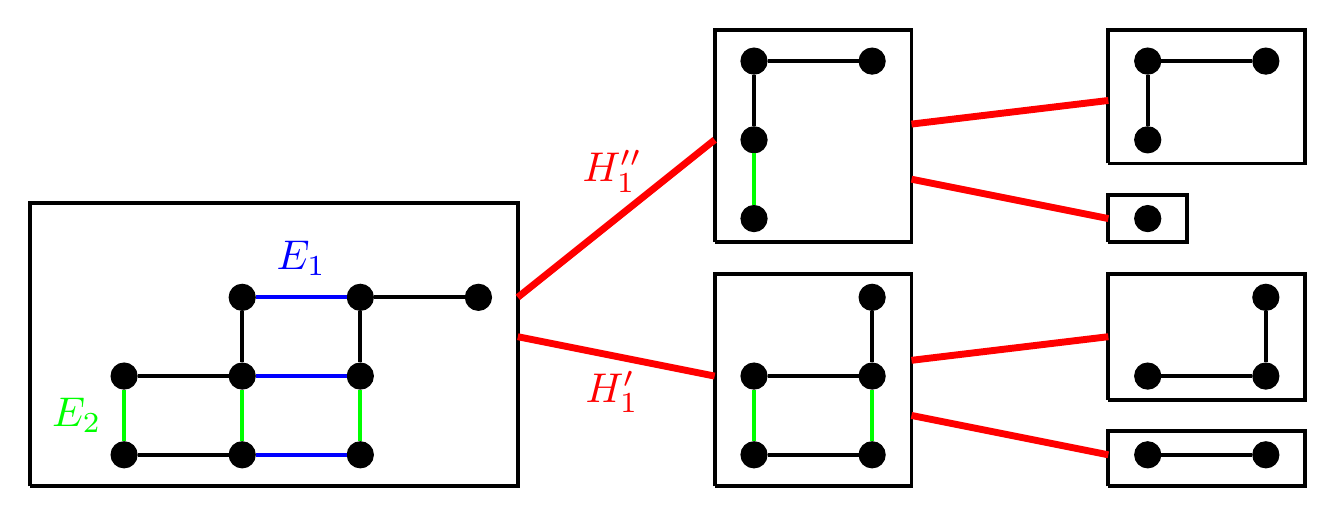
\begin{tikzpicture}

% NODES G1 %%%%%%%%%%%%%%%%%%%%%%%%%%%%%%%%%%%%%%%%%%%%%%%%%%%%%%%%%%%%%%%%%%

\node[draw, circle, minimum height=0.2cm, minimum width=0.2cm, fill=black] (P11) at (1,1) {};
\node[draw, circle, minimum height=0.2cm, minimum width=0.2cm, fill=black] (P12) at (1,2) {};

\node[draw, circle, minimum height=0.2cm, minimum width=0.2cm, fill=black] (P21) at (2.5,1) {};
\node[draw, circle, minimum height=0.2cm, minimum width=0.2cm, fill=black] (P22) at (2.5,2) {};
\node[draw, circle, minimum height=0.2cm, minimum width=0.2cm, fill=black] (P23) at (2.5,3) {};

\node[draw, circle, minimum height=0.2cm, minimum width=0.2cm, fill=black] (P31) at (4,1) {};
\node[draw, circle, minimum height=0.2cm, minimum width=0.2cm, fill=black] (P32) at (4,2) {};
\node[draw, circle, minimum height=0.2cm, minimum width=0.2cm, fill=black] (P33) at (4,3) {};

\node[draw, circle, minimum height=0.2cm, minimum width=0.2cm, fill=black] (P4) at (5.5,3) {};


\draw[line width = 1.4pt, color = green] (P11) -- (P12);
\draw[line width = 1.4pt] (P11) -- (P21);
\draw[line width = 1.4pt] (P12) -- (P22);
\draw[line width = 1.4pt, color = green] (P21) -- (P22);

\draw[line width = 1.4pt, color = blue] (P21) -- (P31);
\draw[line width = 1.4pt, color = blue] (P22) -- (P32);
\draw[line width = 1.4pt, color = green] (P31) -- (P32);

\draw[line width = 1.4pt] (P22) -- (P23);
\draw[line width = 1.4pt, color = blue] (P23) -- (P33);
\draw[line width = 1.4pt] (P32) -- (P33);
\draw[line width = 1.4pt] (P33) -- (P4);

% NODES G2 %%%%%%%%%%%%%%%%%%%%%%%%%%%%%%%%%%%%%%%%%%%%%%%%%%%%%%%%%%%%%%%%%%

\node[draw, circle, minimum height=0.2cm, minimum width=0.2cm, fill=black] (P71) at (9,1) {};
\node[draw, circle, minimum height=0.2cm, minimum width=0.2cm, fill=black] (P72) at (9,2) {};

\node[draw, circle, minimum height=0.2cm, minimum width=0.2cm, fill=black] (P81) at (10.5,1) {};
\node[draw, circle, minimum height=0.2cm, minimum width=0.2cm, fill=black] (P82) at (10.5,2) {};
\node[draw, circle, minimum height=0.2cm, minimum width=0.2cm, fill=black] (P83) at (10.5,3) {};

\draw[line width = 1.4pt, color = green] (P71) -- (P72);
\draw[line width = 1.4pt] (P71) -- (P81);
\draw[line width = 1.4pt, color = green] (P81) -- (P82);
\draw[line width = 1.4pt] (P72) -- (P82);

\draw[line width = 1.4pt] (P82) -- (P83);

% NODES G3 %%%%%%%%%%%%%%%%%%%%%%%%%%%%%%%%%%%%%%%%%%%%%%%%%%%%%%%%%%%%%%%%%%

\node[draw, circle, minimum height=0.2cm, minimum width=0.2cm, fill=black] (P51) at (9,4) {};
\node[draw, circle, minimum height=0.2cm, minimum width=0.2cm, fill=black] (P52) at (9,5) {};
\node[draw, circle, minimum height=0.2cm, minimum width=0.2cm, fill=black] (P53) at (9,6) {};

\node[draw, circle, minimum height=0.2cm, minimum width=0.2cm, fill=black] (P61) at (10.5,6) {};

\draw[line width = 1.4pt, color = green] (P51) -- (P52);
\draw[line width = 1.4pt] (P52) -- (P53);
\draw[line width = 1.4pt] (P53) -- (P61);

% NODES G4 %%%%%%%%%%%%%%%%%%%%%%%%%%%%%%%%%%%%%%%%%%%%%%%%%%%%%%%%%%%%%%%%%%

\node[draw, circle, minimum height=0.2cm, minimum width=0.2cm, fill=black] (P91) at (14,1) {};
\node[draw, circle, minimum height=0.2cm, minimum width=0.2cm, fill=black] (P92) at (15.5,1) {};

\draw[line width = 1.4pt] (P91) -- (P92);

% NODES G5 %%%%%%%%%%%%%%%%%%%%%%%%%%%%%%%%%%%%%%%%%%%%%%%%%%%%%%%%%%%%%%%%%%

\node[draw, circle, minimum height=0.2cm, minimum width=0.2cm, fill=black] (Pa1) at (14,2) {};
\node[draw, circle, minimum height=0.2cm, minimum width=0.2cm, fill=black] (Pa2) at (15.5,2) {};
\node[draw, circle, minimum height=0.2cm, minimum width=0.2cm, fill=black] (Pa3) at (15.5,3) {};

\draw[line width = 1.4pt] (Pa1) -- (Pa2);
\draw[line width = 1.4pt] (Pa2) -- (Pa3);

% NODES G6 %%%%%%%%%%%%%%%%%%%%%%%%%%%%%%%%%%%%%%%%%%%%%%%%%%%%%%%%%%%%%%%%%%

\node[draw, circle, minimum height=0.2cm, minimum width=0.2cm, fill=black] (Pb1) at (14,4) {};

% NODES G7 %%%%%%%%%%%%%%%%%%%%%%%%%%%%%%%%%%%%%%%%%%%%%%%%%%%%%%%%%%%%%%%%%%

\node[draw, circle, minimum height=0.2cm, minimum width=0.2cm, fill=black] (Pc1) at (14,5) {};
\node[draw, circle, minimum height=0.2cm, minimum width=0.2cm, fill=black] (Pc2) at (14,6) {};
\node[draw, circle, minimum height=0.2cm, minimum width=0.2cm, fill=black] (Pc3) at (15.5,6) {};

\draw[line width = 1.4pt] (Pc1) -- (Pc2);
\draw[line width = 1.4pt] (Pc2) -- (Pc3);

% TREE %%%%%%%%%%%%%%%%%%%%%%%%%%%%%%%%%%%%%%%%%%%%%%%%%%%%%%%%%%%%%%%%%%

\draw[line width = 1.4pt] (-0.2,0.6) -- (-0.2,4.2) -- (6.0,4.2) -- (6.0,0.6) -- (-0.2,0.6);
\draw[line width = 1.4pt] (8.5,3.7) -- (8.5,6.4) -- (11.0,6.4) -- (11.0,3.7) -- (8.5,3.7);
\draw[line width = 1.4pt] (8.5,0.6) -- (8.5,3.3) -- (11.0,3.3) -- (11.0,0.6) -- (8.5,0.6);
\draw[line width = 2.5pt, color = red] (6.0,3) -- (8.5,5.0);
\draw[line width = 2.5pt, color = red] (6.0,2.5) -- (8.5,2.0);

\draw[line width = 1.4pt] (13.5,3.7) -- (13.5,4.3) -- (14.5,4.3) -- (14.5,3.7) -- (13.5,3.7);
\draw[line width = 1.4pt] (13.5,4.7) -- (13.5,6.4) -- (16.0,6.4) -- (16.0,4.7) -- (13.5,4.7);
\draw[line width = 1.4pt] (13.5,0.6) -- (13.5,1.3) -- (16.0,1.3) -- (16.0,0.6) -- (13.5,0.6);
\draw[line width = 1.4pt] (13.5,1.7) -- (13.5,3.3) -- (16.0,3.3) -- (16.0,1.7) -- (13.5,1.7);
\draw[line width = 2.5pt, color = red] (11.0,2.2) -- (13.5,2.5);
\draw[line width = 2.5pt, color = red] (11.0,1.5) -- (13.5,1.0);
\draw[line width = 2.5pt, color = red] (11.0,4.5) -- (13.5,4.0);
\draw[line width = 2.5pt, color = red] (11.0,5.2) -- (13.5,5.5);


% ETIQUETTES %%%%%%%%%%%%%%%%%%%%%%%%%%%%%%%%%%%%%%%%%%%%%%%%%%%%%%%%%%%%%%%%%%

\node[color = blue, scale = 1.5] at (3.25,3.5) {$E_1$};
\node[color = green, scale = 1.5] at (0.4,1.5) {$E_2$};

\node[color = red, scale = 1.5] at (7.2,4.6) {$H_1''$};
\node[color = red, scale = 1.5] at (7.2,1.8) {$H_1'$};

\end{tikzpicture}